
\section{Anforderungsspezifikation}
\label{Anforderungsspezifikation}

\subsection{Use Cases}
\label{Anforderungsspezifikation:Use Cases}

Im folgenden sind die funktionalen Anforderungen an das System mit all seinen Komponenten, welche im Kapitel \ref{Architektur} aufgeführt sind, als Use Cases im Brief-Format beschrieben. 
Zur Übersicht ist das Use Case Diagramm in Abbildung \ref{fig:UseCase_OeV-Gueteklassen_2018} zu betrachten.

\begin{figure}[ht]
\centering
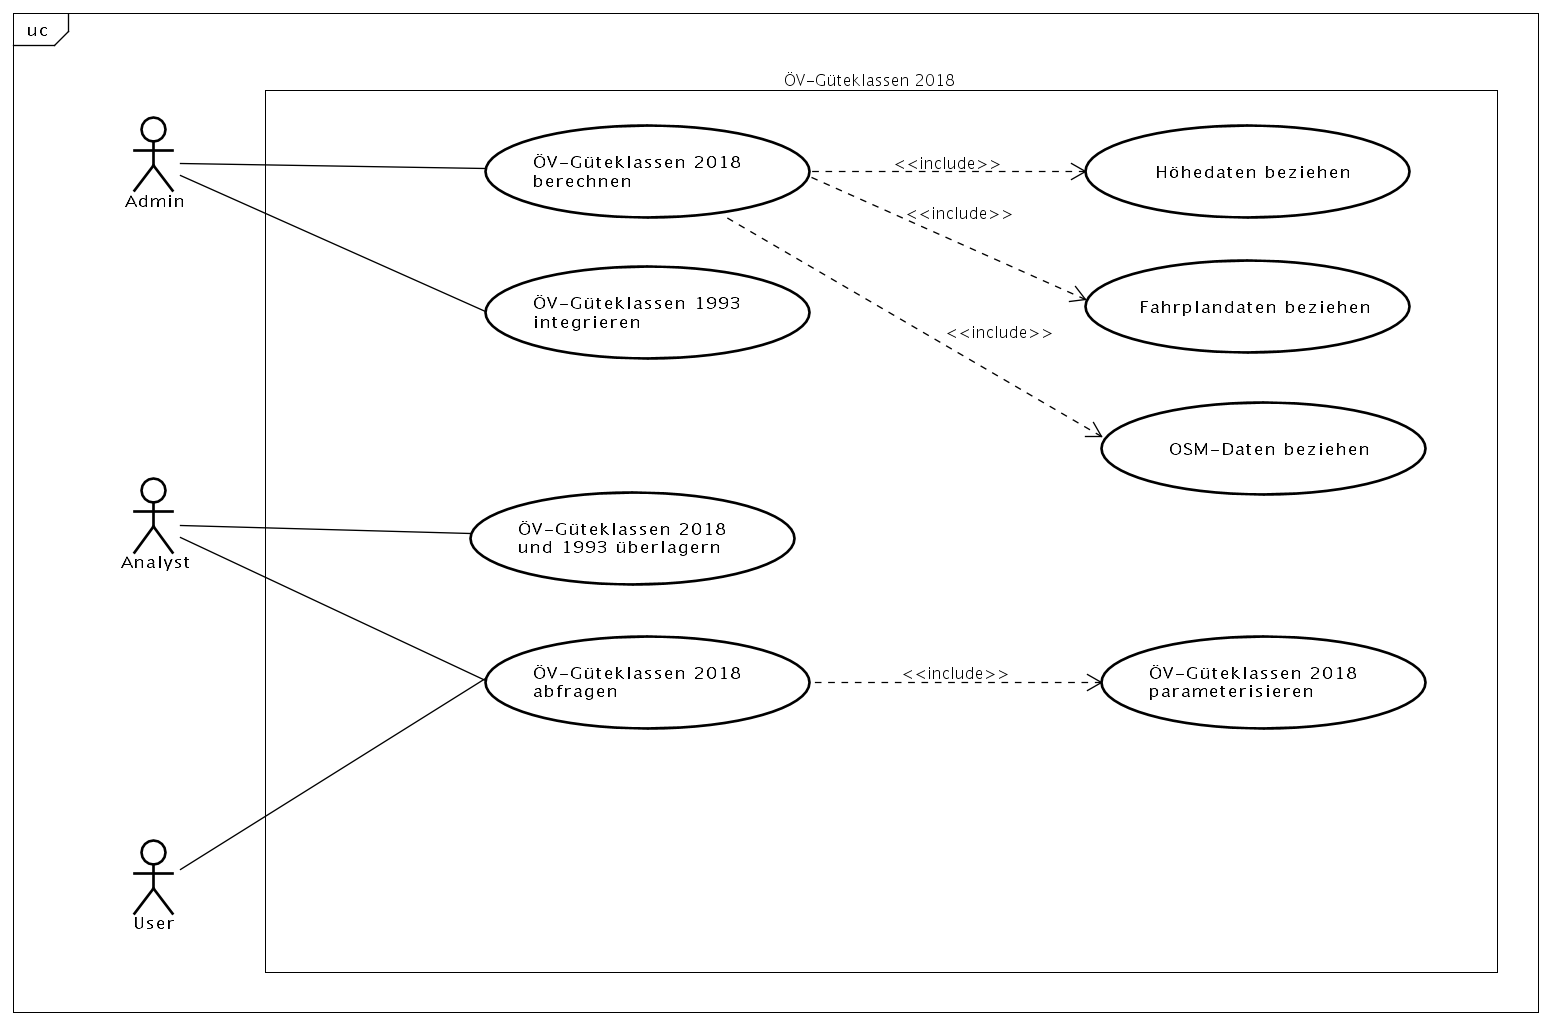
\includegraphics[width=1.0\linewidth]{projectdoc/img/UseCase_OeV-Gueteklassen_2018}
\caption[Use Case Diagramm]{Use Case Diagramm}
\label{fig:UseCase_OeV-Gueteklassen_2018}
\end{figure}

\subsubsection{Aktoren}
\label{Use Cases:Aktoren}

Um die Anforderungen akkurat evaluieren zu können, ist es essentiell dass die Aktoren des Systems identifiziert werden. 
In der Tabelle \ref{table:Aktoren} sind die Aktoren mit ihren Interessen aufgelistet. 

\begin{longtable}{l p{14cm}}
        \toprule
        \textbf{Aktor}
                                & \textbf{Beschreibung und Interesse} \\
        \midrule
        \textbf{Admin}
                                & Ein \emph{Admin} ist für die Bereitstellung von akkuraten \acs{ÖV}-Güteklassen-Daten verantwortlich, welche er den Aktoren \emph{Analyst} und \emph{User} für weitere Auswertung zur Verfügung stellt. So möchte er die erforderlichen Daten sammeln und verarbeiten. \\
        \textbf{Analyst}
                                & Unter dem Aktor \emph{Analyst} sind Raum-/Verkehrsplaner, Transportgesellschaften und weitere Personen, welche die \acs{ÖV}-Güteklassen-Daten für analytische Zwecke und als Planungsinstrument verwenden möchten, zusammengefasst. \\                                
        \textbf{User}
                                & Ein \emph{User} ist grundsätzlich am aktuellen Stand der \acs{ÖV}-Güteklassen in einer bestimmten Region interessiert, welche er als Basis für weitere Entscheidungen bezieht.\\     
                                                     
        \bottomrule
    \caption{Aktoren}
    \label{table:Aktoren}
\end{longtable}

\subsubsection{UC01: TODO}
\label{Use Cases:UC01}

Aktoren: \emph{User}

Include: \nameref{Use Cases:UC02}

%TODO

\subsubsection{UC02: TODO}
\label{Use Cases:UC02}

Aktoren: \emph{User}

%TODO


\subsection{Nicht-funktionale Anforderungen}
\label{Anforderungsspezifikation:Nicht-funktionale Anforderungen}

\subsubsection{NFA01: TODO}
\label{NFA:NFA01}

%TODO

